\chapter{Applications and related problems}\label{chap:Applications}

\section{Applications}\label{sec:Applications}

Set packing has a lot of applications in capital budgeting, crew scheduling, cutting stock, facilities location, graphs and networks, manufacturing, personnel scheduling, districting, information systems, vehicle routing and timetable scheduling, see \cite{Applications} for a survey. In this section some real life applications are mentioned and in Section \ref{sec:RelatedProblems} the relation of set packing to other combinatorial problems is discussed. Section \ref{sec:LocalSearch} then gives some background on local search as a background for Chapter \ref{chap:Results}.

%\subsection{Latin squares and Sudokus}\label{subsec:LatinSquare}

\paragraph{Latin squares} A nice application of set packing is the extension of partial Latin squares \cite{LatinSquare1,LatinSquare2}. A partial Latin square is an $n \times n$ array in which each cell is either empty or coloured with exactly one of the colours $\{1,\ldots,n\}$. A Latin square is a partial Latin square without empty cells where every colour occurs exactly once in every row and every column. The problem is given a partial Latin square to find a completion that colours as many empty cells as possible such that no rows or columns contain any colour more than once.

%Let the universe $\mathcal{U}$ consist of $n^2$ elements of the form $\{e_i, r_j\}$ for every combination of some colour $i$ and some row $j$, $n^2$ elements of the form $\{e_i, c_k\}$ for every combination of some colour $i$ and some column $k$, and $n^2$ elements of the form $\{r_j, c_k\}$ for every combination of some row $j$ and some column $k$.

This can be modeled as a set packing problem as follows. Let the universe $\mathcal{U}$ consist of $3n^2$ elements of the form $\{e_i, r_j\}$, $\{e_i, c_k\}$ and $\{r_j, c_k\}$ for every combination of some colour $i$, some row $j$ and/or some column $k$. Call an element $\{e_i, r_j\}$ or $\{e_i, c_k\}$ empty if respectively row $j$ or column $k$ does not contain colour $i$, and call $\{r_j, c_k\}$ empty if the cell in row $j$ column $k$ is empty. Now let the collection of subsets $\mathcal{C}$ consist of all triplets $\{\{e_i, r_j\}, \{e_i, c_k\}, \{r_j, c_k\}\}$ where all three elements are empty. This creates a set packing instance where every triplet contained in the solution indicates to colour the cell at row $j$ column $k$ with colour $i$. %By the construction of the subsets, every cell is coloured at most once and every row and column contains each colour at most once.

This idea can be extended to the popular Sudoku puzzles. A Sudoku is a $9 \times 9$ Latin square with the additional constraints that in the nine $3 \times 3$ ``boxes'' every colour is allowed only once. Using quadruples rather than triplets, this problem can be translated to set packing in a similar fashion.
%complete a partial Latin square to a Latin square if possible. This can be modeled as a set packing problem as follows. Let the universe $\mathcal{U}$ consist of $n$ elements for every row (so $n^2$ row-elements), $n$ elements for every column (so $n^2$ column-elements), an element for every combination of a row and a colour (so $n^2$ row-colour-elements) and an element for every combination of a column and a colour (so $n^2$ column-colour-elements). Let the subsets in $\mathcal{C}$ be all quadruples of a row-element, a column element, and the colour-elements corresponding to that row and that column. One now needs to find a perfect packing. Since the subsets need to be chosen mutually disjoint, [TODO] [TODO: Figure out how this works]. The given partial Latin square can be incorporated by enforcing the given cells to contain that colour: for every given cell, delete the corresponding quadruples and elements for example.

%Sudoku: We start with the same sets $\mathcal{U}$ and $\mathcal{C}$ as in the previous setting and add $n^2$ elements of the form $\{e_i, b_l\}$ for every combination of some colour $i$ and some block $l$. This element is called empty when colour $i$ does not occur in box $l$. Now extend every triplet $\{\{e_i, r_j\}, \{e_i, c_k\}, \{r_j, c_k\}\}$ to a quadruple with an extra fourth entry $\{e_i, b_l\}$ if the cell at row $j$ column $k$ is in box $l$. Do not extend the other triplets. The set packing instance with the set of all empty quadruples as $\mathcal{C}$ can now be solved to extend the given Sudoku.

\paragraph{Other applications} Three real life applications one could think of is the assignment of crew members to airplanes \cite{Airplanes}, the generation of a coalition structure in multiagent systems \cite{Coalition} and determining the winners in combinatorial auctions to maximise the profit \cite{Auction1,Auction2,Auction3}.

% AIRPLANES A real life application one could think of is the following \cite{Airplanes}. Suppose a fleet of airplanes is given and that every airplane needs a crew consisting of a pilot, a copilot and a navigator. Suppose we are given a set of staff members, and information about their trainings and possible personality conflicts. We need to assign a crew to every airplane such that the trainings for the crew suffice for that airplane and the crew members do not have any personality conflicts.

%We can model this by considering the set of planes and staff members as a universe $\mathcal{U}$ with a collection of subsets $\mathcal{C}$ that represent all possible crew and plane combinations. A maximum packing now represents the maximum possible assignment and ideally we would like a perfect packing where every plane and every crew member has been covered. The essence of the set packing constraint that the subsets need to be mutually disjoint ensures that every element in $\mathcal{U}$ is covered only once, and hence any plane will get at most one crew and no staff member will be assigned to two or more planes.

%\subsection{Coalition structure generation}\label{subsec:Coalition}

% COALITION Another real life application is the generation of a coalition structure in multiagent systems \cite{Coalition}. Given a set of agents $A$, a coalition structure is a partitioning of $A$ into disjoint exhaustive subsets. Every agent is thus in exactly one coalition. Every possible coalition $C$ is associated with a value $v_C$ and the objective is to find a coalition structure $S$ maximizing its value $\sum_{C \in S} v_C$. %In most applications the set of agents and possible coalitions are huge and there are limited resources or time to exhaustively search this space. When we do not care about the identity of every agent and we only need to consider the value $v_C$ of every coalition, this problem is equivalent to the weighted set packing problem.

%\subsection{Combinatorial auctions}\label{subsec:Auctions}

% AUCTION A third real life application is determining the winners in a combinatorial auction so as to maximize the total revenue \cite{Auction1,Auction2,Auction3}. Combinatorial auctions are auctions in which a number of items are up for sale and bidders can bid for combinations of items. If we consider the set of items as the universe $\mathcal{U}$ and the set of all bids to be $\mathcal{C}$, this translates to the set packing problem where we need to determine the winners to make the most profit. %Auction theory is a subfield of game theory that has drawn some attention for the past few decades.

\section{Related problems}\label{sec:RelatedProblems}

Set packing is highly related to the hypergraph matching problem and the independent set problem. This section surveys these relations and some special cases of set packing.

\subsection{Hypergraph matching}\label{subsec:Hypergraphs}

Set packing and hypergraph matching are really the same problem with different names. This subsection contains some background on hypergraphs and hypergraph matchings and relates these notions to set packing and $k$-set packing.

\paragraph{Hypergraphs} A hypergraph $H$ is a pair $H=(V,E)$ where $V$ is the set of vertices and $E$ is the set of hyperedges. A hyperedge $e \in E$ is a nonempty subset of the vertices. In a weighted hypergraph, every hyperedge $e \in E$ is associated with a weight $w(e)$. A hyperedge $e \in E$ is said to contain, cover or be incident to a vertex $v \in V$ when $v \in e$.

For a vertex $v$, $\delta(v)$ denotes the set of hyperedges incident to it. The degree of a vertex $v$ is $|\delta(v)|$. %We say two vertices $u$ and $v$ are adjacent when there is a hyperedge $e \in E$ containing both $u$ and $v$. There might be multiple hyperedges touching the same set of vertices.
The cardinality of a hyperedge is the number of vertices it contains. When every vertex has the same degree $k$, the hypergraph is called $k$-regular. When every hyperedge has the same cardinality $k$, the hypergraph is $k$-uniform. A graph is thus a 2-uniform hypergraph. In a graph, every edge is a subset of two vertices.

\paragraph{Matchings} A hypergraph matching is a subset of the hyperedges $M \subseteq E$ such that every vertex is covered at most once, i.e. the hyperedges are mutually disjoint. This generalises matchings in graphs. From now on, with matching we mean a hypergraph matching. The cardinality of a matching is the number of hyperedges it contains. %A matching $M$ is called maximal if there is no hyperedge $e \in E \setminus M$ such that $M \cup \{e\}$ is a matching.
A matching is called maximum if it has the largest cardinality of all possible matchings. %A matching is called perfect if every vertex is covered exactly once.
In the hypergraph matching problem, a hypergraph is given and one needs to find the maximum matching.
%
\begin{quote}
\begin{bf}Hypergraph matching problem\end{bf}\\
Given: a hypergraph $H = (V,E)$ \\
Find: a maximum collection of mutually disjoint hyperedges.
\end{quote}
%
%We call a hypergraph bipartite when the vertices can be partitioned into two sets $U$ and $V$ such that every hyperedge is incident to exactly one vertex from $U$. We say a bipartite matching is perfect if every vertex in $U$ is covered exactly once. %In the Santa Claus problem treated in Subsection \ref{subsec:SantaClaus} we were actually considering a bipartite hypergraph with $U$ as the set of players and $V$ the set of the resources. The problem was really to find a perfect bipartite matching in this hypergraph.
\paragraph{$k$-partite hypergraphs}
The notion of bipartiteness in graphs can be generalised in a hypergraph to the concept of $k$-partiteness. A hypergraph $H = (V,E)$ is called $k$-partite if the set of vertices $V$ can be partitioned into $k$ classes $V_1, \ldots, V_k$ such that every hyperedge $e \in E$ touches exactly one vertex from every vertex class. A $k$-partite hypergraph is $k$-uniform by definition. The hypergraph matching problem on a $k$-partite graph is also called the $k$-dimensional matching problem. This generalises the bipartite matching on graphs where $k=2$ and it is a restricted version of hypergraph matching on a $k$-uniform hypergraph. In particular the 3-dimensional matching problem is well studied in literature. %[TODO] [TODO: add citations].

\paragraph{Relation to set packing} Let a set packing instance $S = (\mathcal{U},\mathcal{C})$ be given. Define a hypergraph $H = (\mathcal{U}, \mathcal{C})$, calling the elements in $\mathcal{U}$ vertices and the subsets in $\mathcal{C}$ hyperedges. Then the set packing problem on $S$ is exactly the same as the hypergraph matching problem on $H$. An instance of the $k$-set packing problem translates to an instance of the hypergraph matching problem on a $k$-uniform hypergraph, as every subset (hyperedge) contains exactly $k$ elements. %This is a generalization of the well-known graph matching where $k=2$. %Even though for the case of $k=2$ the maximum cardinality and even the maximum weight matching can be found in polynomial time, already for $k=3$ the problem becomes NP-hard.

Results for set packing thus immediately apply to hypergraph matching and vice versa.

%\subsection{Santa Claus problem}\label{subsec:SantaClaus}
%
%A nice problem related to set packing is the Santa Claus problem, also known as the max-min fair allocation problem \cite{SantaClaus1,SantaClaus2,SantaClaus3}. In this problem, there is a set of resources $\mathcal{R}$ and a set of players $\mathcal{P}$. Every player $p$ has a specific value $p(r)$ for any resource $r$. The goal in the Santa Claus problem is to allocate the resources to the players in order to maximize the minimum of the sum of the values of the resources given to any player, i.e. to make the least happy player as happy as possible. When every resource has a fixed value for any player (i.e. $p(r)$ is the same for all players $p$), the problem is known as the restricted Santa Claus problem or the restricted max-min fair allocation problem.
%%
%\begin{quote}
%\begin{bf}Restricted Santa Claus problem\end{bf}\\
%Given: a set of players $\mathcal{P}$, a set of resources $\mathcal{R}$ and a weight function $w:\mathcal{R} \rightarrow \mathbb{R}$ \\
%Find: an allocation $m:\mathcal{R} \rightarrow \mathcal{P}$ of the resources to the players maximizing $\min_{p \in \mathcal{P}} \sum_{r \in m^{-1}(p)} w(r)$. [TODO: equationform]
%\end{quote}
%
%One can model this as a set packing problem as follows, using a binary search on the objective value $v$. For a fixed value $v$, one needs to check whether it is possible to assign a subset of the resources of at least value $v$ to every player. If this is possible, one can check for a higher value of $v$. It suffices to consider only subsets of resources that are minimal in the sense that leaving out any resource lowers its value to below $v$: it does not make sense to assign more resources to a player than needed for objective value $v$. This is easily translated to set packing: let the universe $\mathcal{U}$ contain all resources and all players once and let the collection $\mathcal{C}$ contain all minimal subsets containing one player and a set of resources whose total value is at least $v$. If it is possible to find as many mutually disjoint subsets as the number of players, the objective value $v$ can be reached.

%One can model this restricted problem as a weighted hypergraph matching problem as follows, using a binary search on the objective value $v$. For a fixed value $v$, one needs to check whether it is possible to assign a subset of the resources of at least value $v$ to every player. If this is possible, one can check for a higher value of $v$. It suffices to consider only subsets of resources that are minimal in the sense that leaving out any resource lowers its value to below $v$: it does not make sense to assign more resources to a player than needed for objective value $v$. This is easily translated to weighted hypergraph matching: let a hypergraph contain one vertex for every resource and every player and create a hyperedge for every minimal subset containing one player and a set of resources whose total value is at least $v$. If there exists a perfect matching in this hypergraph (covering every player), the objective value $v$ can be reached.

%One can model this restricted problem as a weighted hypergraph matching problem as follows. It uses a binary search on the objective value. For a given value $v$, every player needs to be assigned a subset of the resources of at least value $v$. We can now create a bipartite hypergraph, which contains a vertex for every player and every resource, and every hyperedge connects exactly one player to some subset of the resources of at least value $v$. Create hyperedges for all such subsets. If there exists a perfect matching in this hypergraph, there is an allocation of value $v$, where a perfect matching is a set of hyperedges such that every player is in one of these hyperedges. This problem is thus highly related to the (bipartite) hypergraph matching problem and hence to the set packing problem.

\subsection{Independent set}\label{subsec:IndependentSet}

\paragraph{Relation to set packing} Set packing is also closely related to the (maximum) independent set problem. Given a graph $G = (V,E)$, an independent set is a subset of vertices that are mutually non-adjacent, i.e. a set of vertices whose induced subgraph does not contain any edge. This subsection treats this problem and its relation to set packing.
%
\begin{quote}
\begin{bf}Independent set problem\end{bf}\\
Given: a graph $G = (V,E)$ \\
Find: a maximum collection of mutually non-adjacent vertices.
\end{quote}
%
Let a set packing instance $I = (\mathcal{U},\mathcal{C})$ be given. Create the conflict graph $G = (\mathcal{C},E)$ %with a vertex for every subset in $\mathcal{C}$ and an edge between two vertices $S, T \in \mathcal{C}$ when the two subsets these vertices correspond to are not disjoint (i.e. $S \cap T \neq \emptyset$).
for the instance $I$. Then the edge set $E$ captures all the intersections between the subsets. Any packing of $\mathcal{C}$ now corresponds to an independent set in $G$: as a packing is mutually disjoint by definition, the corresponding vertices are non-adjacent. On the other hand, any independent set in $G$ corresponds to a packing of $\mathcal{C}$. Finding a maximum packing is thus equivalent to finding a maximum independent set in the conflict graph.

\paragraph{Relation to $k$-set packing} Now consider a $k$-set packing instance $(\mathcal{U}, \mathcal{C})$ where every subset in $\mathcal{C}$ contains exactly $k$ elements from $\mathcal{U}$. Consider a fixed subset $S$ and look at the set $N(S)$ of all subsets intersecting $S$. There can be at most $k$ subsets in $N(S)$ that are mutually disjoint, when each subset intersects $S$ in a distinct element. Thus within $N(S)$, the maximum packing has at most cardinality $k$.

Now consider the corresponding conflict graph $G$. $S$ is a vertex in $G$ and $N(S)$ is the set of all neighbours of $S$. By the previous reasoning, $N(S)$ contains an independent set of size at most $k$. Thus in the neighbourhood of any vertex of $G$ there are at most $k$ mutually non-adjacent vertices. In other words, the conflict graph is $k+1$-claw free: it does not contain $K_{1,k+1}$ as an induced subgraph, where $K_{n,m}$ is the complete bipartite graph on $n$ and $m$ vertices. A vertex can have any number of neighbours, but the maximum number of mutually non-adjacent neighbours is $k$. %When the cardinality of every subset is bounded by $k$, the conflict graph in which we need to find an independent set thus inherits this property.

% [TODO] This is not right! W_8 can be the conflict graph of some instance of 14-SP, just create an element for every edge?

%It should be noted that the maximum independent set problem in $k+1$-claw free graphs is a more general problem than $k$-set packing \cite{ThesisChan}. Consider the cycle graph $C_{2k+1}$ and add a center vertex connected to all vertices to create the wheel graph $W_{2k+2}$ (see Figure \ref{fig:WheelGraph} for the case $k=3$). Since the center vertex is connected to every vertex, any independent set in this graph consists of at most $k$ vertices. We claim there is no instance of $k$-set packing having this intersection graph. The largest complete subgraph is a triangle, consisting of the center of the wheel and two consecutive elements on the cycle. Distinct triangles cannot cover the same elements, because otherwise there would be another edge in the intersection graph. Two consecutive triangles share one edge and hence one element for two sets. But there are $2k+1$ triangles and there are only $k$ elements, so there is no $k$-set packing instance with this intersection graph.

%\begin{figure}
%        \centering
%        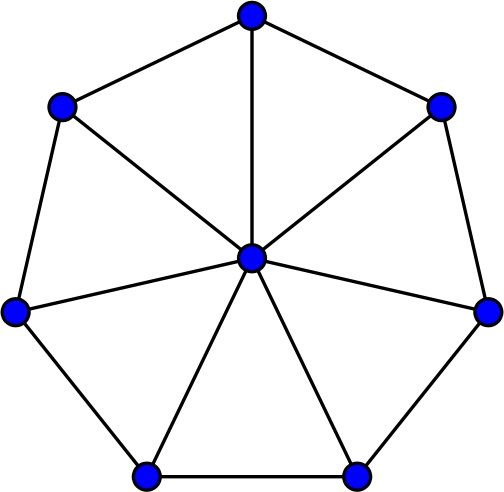
\includegraphics[width = 0.3 \textwidth]{Images/WheelGraph.jpg}
%        \caption{The wheel graph $W_8$. There is no instance of 3-SP with $W_8$ as an intersection graph.}
%        \label{fig:WheelGraph}
%\end{figure}

%\begin{figure}
%\centering
%\begin{tikzpicture}
%\node[draw, circle] at (0,0) {};
%\foreach \s in {1,...,7}
%{
%  \node[draw, circle] at ({360/7 * (\s - 1)}:3cm) {};
%  \draw[>=latex] ({360/7 * (\s - 1)+8}:3cm)
%    arc ({360/7 * (\s - 1)+8}:{360/7 * (\s)-8}:3cm);
%  \draw[>=latex] (0,0) arc ({360/7 * (\s - 1)+8}:{360/7 * (\s)-8}:3cm);
%}
%\end{tikzpicture}
%\caption{The wheel graph $W_8$. There is no instance of 3-SP with $W_8$ as an intersection graph.}
%        \label{fig:WheelGraph}
%\end{figure}

\paragraph{Independent set on bounded degree graphs} On the other hand, the maximum independent set problem in graphs $G$ where all degrees are bounded by $k$ is a special case of $k$-set packing. Map every vertex in $G$ to a subset in $\mathcal{C}$ and map every edge to a distinct element in $\mathcal{U}$. Let a subset in $\mathcal{C}$ (a vertex in $G$) contain all elements in $\mathcal{U}$ (edges in $G$) that are incident to it. Now every subset in $\mathcal{C}$ contains at most $k$ elements because every vertex in $G$ had degree at most $k$. Again, by adding dummy elements to the subsets with less than $k$ elements, every subset in $\mathcal{C}$ has exactly $k$ elements. As such, the $k$-set packing problem generalises the maximum independent set problem on bounded degree graphs.

Section \ref{sec:IS} discusses the relation between the results on set packing and independent set more thoroughly.
%As such, the $k$-set packing problem generalizes the maximum independent set problem in bounded degree graphs. This is an NP-complete problem, it does not admit a polynomial time approximation scheme \cite{noPTAS1}, and assuming the Unique Games conjecture (see \cite{UGC}) the problem of finding a maximum independent set in a $d$-regular graph cannot be approximated within a factor $O\left(\frac{d}{\log^2{d}}\right)$ \cite{Bounded1}. On the positive side, the greedy approach for this problem was shown to have an approximation ratio of $\frac{d+2}{3}$ \cite{GreedIsGood}. The currently best approximation algorithm achieves an approximation guarantee of $O\left(\frac{d}{\log \log d}\right)$ \cite{Bounded2}. In Chapter \ref{chap:IS} we will elaborate more on the difference between the maximum independent set problem in bounded degree graphs and $k+1$-claw free graphs [TODO].

%\subsection{Covering and packing problems}\label{subsec:CoveringProblems}
%
%Set packing is one of the standard packing problems, which are closely related to covering problems. Roughly speaking, in a packing problem one needs to find a maximum set such that every element is packed at most once, while in a covering problem one needs to find a minimum set such that every element is covered at least once. In fact, the LP-dual of a packing problem is a covering problem in general and vice versa. Table \ref{tab:PackingCovering} lists some of these LP-dualities. We refer to \cite{Reductions} for a survey of these problems.
%%
%\begin{table}
%\centering
%\begin{tabular}{ll}
%  \toprule
%  \multicolumn{2}{c}{Covering-packing dualities} \\
%  \midrule
%  Minimum set cover    & Maximum set packing \\
%  Minimum vertex cover & Maximum matching \\
%  Minimum edge cover   & Maximum independent set \\
%  \bottomrule
%\end{tabular}
%\caption{Every horizontal pair of problems are each other's LP-duals.}
%\label{tab:PackingCovering}
%\end{table}

%The LP-dual of (maximum) set packing is minimum set cover, which is the following problem. It should be noted that due to duality, any solution to Minimum Set Cover is an upper bound to the maximum set packing.
%%
%\begin{quote}
%\begin{bf}Minimum Set Cover\end{bf}\\
%Given: a universe $\mathcal{U}$, a collection $\mathcal{C}$ of subsets over $\mathcal{U}$ \\
%Find: a minimum subcollection $\mathcal{S} \subseteq \mathcal{C}$ whose union is $\mathcal{U}$.
%\end{quote}
%%
%Set cover is equivalent to the hitting set problem, which is the following.
%%
%\begin{quote}
%\begin{bf}Minimum Hitting Set\end{bf}\\
%Given: a universe $\mathcal{U}$, a collection $\mathcal{C}$ of subsets over $\mathcal{U}$ \\
%Find: a minimum set $\mathcal{T} \subseteq \mathcal{U}$ for which $T \cap S \neq \emptyset$ for all $S \in \mathcal{C}$.
%\end{quote}
%%
%So in the minimum set cover problem, we are searching for a collection of subsets that touches every element at least once. In the minimum hitting set problem, we are searching for a set of vertices that touches every subset at least once. These problems are the same. Consider an instance for set cover with $\mathcal{U} = \{u_1, \ldots, u_n\}$. Now define $\mathcal{T}_i = \{S \in \mathcal{C} \mid u_i \in S\}$, i.e. the set of subsets that contain the element $u_i$. Define $\mathcal{X} = \{\mathcal{T}_1, \ldots, \mathcal{T}_n\}$ as the set of all these sets. Then $(\mathcal{C},\mathcal{X})$ is an equivalent hitting set instance: every vertex in the hitting set instance is a subset in $\mathcal{C}$, and a set of such vertices that touches every edge at least once is a set of subsets in $\mathcal{C}$ that touches every element in $\mathcal{U}$ at least once by the definition of $T_i$. Equivalently, a minimum set cover in $(\mathcal{U},\mathcal{C})$ implies a hitting set in $(\mathcal{C},\mathcal{X})$: every subset in the set cover instance is a vertex in $\mathcal{U}$, and a set of such subsets that touches every element at least once is a set of vertices in $\mathcal{U}$ that touches every edge in $X$ at least once.
%
%These problems can also be formulated in terms of hypergraphs. In the minimum set cover problem, we are looking for a minimum collection of hyperedges that covers every vertex. In the minimum hitting set problem, we are looking for a minimum collection of vertices that touches every hyperedge.
%
%A special case of the set cover problem is the vertex cover problem \cite{Paschos}.
%%
%\begin{quote}
%\begin{bf}Minimum Vertex Cover\end{bf}\\
%Given: a graph $G = (V,E)$ \\
%Find: a minimum subset $S \subseteq V$ such that $e \cap S \neq \emptyset$ for all $e \in E$.
%\end{quote}
%%
%So in the minimum vertex cover problem, we are searching for a minimum set of vertices that touches every edge at least once. Indeed, a vertex cover instance is just a hitting set instance where every subset has cardinality 2 (being a pair rather than a subset over $\mathcal{U}$, or being an edge rather than a hyperedge). A hitting set is just a vertex cover in a hypergraph instead of a graph. Since hitting set and set cover are equivalent, vertex cover is indeed a special case of set cover. The dual of the problem asks for a maximum set of edges that touches every vertex at most once, i.e. the matching problem. Indeed, this is a special case of the hypergraph matching problem, which is the dual problem of set cover.
%
%Another special case of set cover is edge cover.
%%
%\begin{quote}
%\begin{bf}Minimum Edge Cover\end{bf}\\
%Given: a graph $G = (V,E)$ \\
%Find: a minimum subset $T \subseteq E$ whose union is $V$.
%\end{quote}
%%
%So in the minimum edge cover problem, we are searching for a minimum set of edges that touches every vertex at least once. Indeed, an edge cover instance is just a set cover instance where every subset has cardinality 2. A set cover is just an edge cover in a hypergraph. The dual of the problem asks for a maximum set of vertices that touches every edge at most once, i.e. the independent set problem.

%\paragraph{Hardness results} Set packing is the dual of set cover, these two problems are the most general of the problems mentioned here. There are close connections between the problems, and connections with hypergraphs. The edge cover problem and the matching problem are the only problems that can be solved in polynomial time \cite{noPTAS2}. The following results on the hardness of the problems also apply to the set packing problem. Arora et al showed that, unless $\mathcal{P} = \mathcal{NP}$, the vertex cover does not admit a polynomial time approximation scheme, even on bounded degree graphs \cite{noPTAS1}. Moreover, also assuming that $\mathcal{P} \neq \mathcal{NP}$, it has been shown that there is no constant-ratio polynomial time approximation scheme for independent set \cite{noPTAS2,NoPTAS3}. H{\aa}stad proved that set packing cannot be approximated within $n^{1 - \varepsilon}$, where $n$ is the number of sets, unless $\mathcal{NP} \subseteq \mathcal{ZPP}$ \cite{CliqueIsHard}.

%Even though these hardness results might seem strong, there have been quite some results on the positive side, which are treated in Chapter \ref{chap:Results}. As a lot of these results use local search techniques, first some background about this area is given. %Also, the dual problem of set packing is the classical set cover problem (see e.g. \cite{SetCover1,SetCover2}) which generalizes the vertex cover problem mentioned before \cite{Paschos}.

\subsection{Special cases of set packing}

\paragraph{Clique and triangle packing} There are some special cases of set packing we would like to mention. Instead of studying the set packing problem with a bound on the cardinality of every subset, it is also possible to study the problem with certain given structures on the given sets. One example is the clique packing problem, where one is given some graph $G$. A packing of $G$ is a collection of pairwise vertex-disjoint subgraphs of $G$, each of which is isomorphic to a clique. A packing is said to cover an edge of $G$ if one of the subgraphs contains that edge. In the clique packing problem, one tries to maximise the number of covered edges \cite{CliquePacking}. The special case where every clique is of size 3 is called the triangle packing problem \cite{TrianglePacking2,TrianglePacking1}. The set packing problem generalises these problems.

%\subsection{Tree-like weighted set packing}\label{subsec:TreeLike}

\paragraph{Tree-like weighted set packing} The tree-like weighted set packing problem is another subproblem with an additional structure on the sets that allows for better results that even extend to the weighted version. In this problem, the subsets in $\mathcal{C}$ can be organised into a forest $F$ satisfying the following properties. Every vertex in $F$ corresponds to one subset in $\mathcal{C}$. If a vertex $Y$ is a child of a vertex $X$, then $Y$ is a subset of $X$. If $Y$ and $Z$ are distinct children from $X$, then $Y$ and $Z$ are disjoint. And the roots of all the trees are pairwise disjoint. When the sets are structured like this, the problem can be solved exactly in cubic time using a dynamic programming algorithm \cite{TreeSP}.

\paragraph{$k$-dimensional matching} Perhaps the best known special case of $k$set packing is the $k$-dimensional matching problem. As was mentioned in Subsection \ref{subsec:Hypergraphs}, this is the hypergraph matching problem on a $k$-partite hypergraph, which is a stronger structure than a $k$-uniform hypergraph. In particular 3-dimensional matching is well-known. All results for $k$-set packing immediately apply to $k$-dimensional matching. %and there are some results specifically for $k$-dimensional matching that exploit this extra structure.

%Some subproblems with additional structure on either the structure or the weights of the sets allow for better results. One example is the tree-like weighted set packing problem. In this problem, the subsets in $\mathcal{C}$ can be organized into a forest $F$ satisfying the following properties. Every vertex in $F$ corresponds to one subset in $\mathcal{C}$. If a vertex $Y$ is a child of a vertex $X$, then $Y$ is a subset of $X$. If $Y$ and $Z$ are distinct children from $X$, then $Y$ and $Z$ are disjoint. And the roots of all the trees are pairwise disjoint. When the sets are structured like this, the problem can be solved exactly in cubic time using a dynamic programming algorithm \cite{TreeSP}.

%The weighted set packing problem can also be approximated better when the weights of the set are structured like the following: every element $u$ in $\mathcal{U}$ is associated with a weight $w(u)$ and the weight of any subset in $\mathcal{C}$ is the sum of the weights of the elements it contains. In this case, there is an approximation algorithm for this problem within a factor of $O(\frac{n}{\log n})$ \cite{SpecialWeight}. [TODO] [TODO: This is not true, IS on hypergraphs is defined differently in this paper so other problem?!]

\section{Local search}\label{sec:LocalSearch}

\paragraph{Background} A lot of the approximation algorithms for $k$-set packing are related to the notion of local search techniques. In this section we survey this related topic. Local search is a natural heuristic to tackle difficult problems. The most basic solution approaches for a discrete optimization problem are generating just one solution (e.g. using a priority-based heuristic), enumerating implicitly all possible solutions (e.g. with branch and bound techniques) and generating several solutions and choosing the best. Local search is a heuristic that finds from an initial solution a sequence of solutions that use the previous solution for the next solution, with the goal to increase the objective value from the initial solution to a better value. A neighbourhood structure is defined on the solutions that somehow resembles similar solutions. Until some stopping criterion is reached, in every iteration a solution from the neighbourhood of the current solution is chosen.

A local search heuristic usually consists of four main elements: a method to calculate an initial solution, a definition of the neighbourhood of a solution, a criterion to choose a solution from any neighbourhood, and a stopping criterion. The method to calculate an initial solution is needed to start a local search, but is usually not seen as a part of the local search technique itself. For example, Chapter \ref{chap:Results} contains a lot of results stating that a locally optimal solution with respect to some neighbourhood structure achieves a certain approximation guarantee, without going into the details of how to find an initial solution or sometimes even how to iterate to the next solution.

\paragraph{Results} Local search techniques are widely used in practice, the most common example being for the traveling salesman problem. However, there are not much positive results on local search in theory. In fact, a complexity class called $\mathcal{PLS}$ (polynomial time local search) has been defined \cite{PLS}. Problems that are $\mathcal{PLS}$-complete are as hard as the hardest local optimization problems. A lot of well-known heuristics are known to be $\mathcal{PLS}$-complete. There are even some problems for which it has been proved that there is no sequence, of less than exponential length, of improvements ending in a locally optimal solution \cite{Halldorsson}. To make matters worse, there are popular heuristics with good average-case behaviour that perform quite bad at relatively easy problems. For instance, the algorithm at the heart of the well-known simulated annealing performs quite poor at finding a maximum matching (which is even in $\mathcal{P}$).

On the positive side, set packing does not fit this negative theoretic framework. Currently all approximation algorithms for both the weighted and the unweighted $k$-set packing problem use local search at their core. %In \cite{Halldorsson} a lot of results are mentioned on different problems, all using local search.
However, there are also some results on the limits of the approximation guarantees using local search.
The next chapter proceeds with approximation algorithms for $k$-set packing %, which are all closely related to the framework of local search,
and the bounds on what is achievable using this technique. %To make sure no confusion may arise we first define some notation and definitions. 